% EE 513 Project 1 
\documentclass[9pt]{extarticle}
\usepackage[letterpaper,margin=0.6in]{geometry}
\usepackage[T1]{fontenc}
\usepackage[utf8]{inputenc}
\usepackage[scaled=0.95]{helvet}
\renewcommand{\familydefault}{\sfdefault}
\usepackage{amsmath,amssymb}
\usepackage{graphicx}
\usepackage{booktabs,tabularx,array}
\usepackage{xcolor}
\usepackage[most]{tcolorbox}
\usepackage{enumitem}
\usepackage[font=footnotesize,labelfont=bf,skip=2pt]{caption}
\usepackage{titlesec}
\usepackage[section]{placeins}
\usepackage[hidelinks]{hyperref}

\definecolor{muted}{HTML}{4A5560}
\definecolor{warnbg}{HTML}{FDF3E7}\definecolor{warnbar}{HTML}{C77A12}
\definecolor{notebg}{HTML}{F3F5F7}\definecolor{notebar}{HTML}{8A96A3}
\newtcolorbox{note}{enhanced,colback=notebg,colframe=notebg,borderline west={2.5pt}{0pt}{notebar},
  sharp corners,boxrule=0pt,left=6pt,right=6pt,top=3pt,bottom=3pt,fontupper=\small}
\newtcolorbox{warn}{enhanced,colback=warnbg,colframe=warnbg,borderline west={2.5pt}{0pt}{warnbar},
  sharp corners,boxrule=0pt,left=6pt,right=6pt,top=3pt,bottom=3pt,fontupper=\small}

\makeatletter
\newenvironment{textfig}[3][0.55]{%
  \def\tf@file{#2}\def\tf@cap{#3}\def\tf@w{#1}%
  \par\noindent\begin{minipage}[t]{\tf@w\linewidth}\vspace{0pt}}%
 {\end{minipage}\hfill
  \begin{minipage}[t]{\dimexpr0.97\linewidth-\tf@w\linewidth\relax}\vspace{0pt}\centering
  \includegraphics[width=\linewidth]{figures/\tf@file}\captionof{figure}{\tf@cap}\end{minipage}\par\medskip}
\makeatother
\newcommand{\todo}[1]{\textcolor{red}{[#1]}}

\titleformat{\section}{\large\bfseries}{\thesection}{0.6em}{}[\vspace{-4pt}\rule{\linewidth}{0.8pt}]
\titlespacing*{\section}{0pt}{8pt}{4pt}
\titleformat{\subsection}{\normalsize\bfseries}{}{0em}{}
\titlespacing*{\subsection}{0pt}{6pt}{2pt}
\setlength{\parindent}{0pt}\setlength{\parskip}{3pt}
\setlist{nosep,leftmargin=14pt}
\setlength{\textfloatsep}{6pt}\setlength{\floatsep}{6pt}\setlength{\intextsep}{6pt}
\pagestyle{plain}

\begin{document}

{\LARGE\bfseries iPhone 17 Pro Max Main Camera Characterization Datasheet}\par\vspace{3pt}
{\small\color{muted}
\textbf{\color{black}Andrei Perez} \quad EE 513 Project 1, Fall 2026\\
\textbf{\color{black}Repository:} \url{https://github.com/anfepel/ee513}\\
\textbf{\color{black}Camera:} iPhone 17 Pro Max back camera 6.765mm f/1.78, raw Bayer DNG (BGGR, 12-bit, black 528 DN, white 4095 DN) with 4032$\times$3024 output (48 MP sensor, 2$\times$2 binned), captured with Adobe Lightroom at 1$\times$, no zoom. Camera verified with the \texttt{lens\_id} assertion on all 65 files.}

\vspace{4pt}
{\small
\renewcommand{\arraystretch}{1.15}
\begin{tabularx}{\linewidth}{@{}>{\raggedright\arraybackslash}p{0.12\linewidth}>{\raggedright\arraybackslash}p{0.22\linewidth}>{\raggedright\arraybackslash}p{0.33\linewidth}>{\raggedright\arraybackslash}X@{}}
\toprule
\textbf{Measurement} & \textbf{Quantity} & \textbf{Value $\pm$ 1$\sigma$} & \textbf{How obtained / note} \\ \midrule
\textbf{Geometry} & Focal length $f_x$, $f_y$ & 2924.8\,$\pm$\,14.1, 2927.4\,$\pm$\,13.6 px & \textcolor{muted}{\scriptsize Zhang, 17 views; $\sigma$ = max(OpenCV, jackknife)} \\
\textbf{} & Focal length (mm) & 7.08\,$\pm$\,0.15 mm (EXIF 6.765) & \textcolor{muted}{\scriptsize $f_x\times$ pitch; pitch bound $\pm$2.1\,\%} \\
\textbf{} & Principal point $c_x$, $c_y$ & 2024.1\,$\pm$\,4.3, 1513.5\,$\pm$\,4.0 px & \textcolor{muted}{\scriptsize image centre 2016, 1512} \\
\textbf{} & Radial $k_1$, $k_2$ ($k_3=0$) & $+$0.182\,$\pm$\,0.006, $-$0.522\,$\pm$\,0.038 & \textcolor{muted}{\scriptsize valid only for $r\le1442$ px (57\,\% of corner radius)} \\
\textbf{} & Tangential $p_1$, $p_2$ & $-$0.0023\,$\pm$\,0.0006, $-$0.0008\,$\pm$\,0.0006 & \textcolor{muted}{\scriptsize } \\
\textbf{} & RMS reprojection error & 0.665\,$\pm$\,0.054 px & \textcolor{muted}{\scriptsize 17/19 views detected} \\ \midrule
\textbf{MTF} & MTF50, centre & 0.285\,$\pm$\,0.021 cy/px$_g$ = 59\,$\pm$\,4 cy/mm & \textcolor{muted}{\scriptsize = 0.57 $\times$ Nyquist (0.5); $n$ = 10} \\
\textbf{} & MTF50, off-axis squares ($r$ = 0.36--0.47) & TL 0.170\,$\pm$\,0.013\newline TR 0.224\,$\pm$\,0.021\newline BL 0.188\,$\pm$\,0.014\newline BR 0.234\,$\pm$\,0.021 & \textcolor{muted}{\scriptsize mean/centre = 0.72\,$\pm$\,0.02; true frame corners not reached} \\
\textbf{} & MTF at green Nyquist, centre & 0.205\,$\pm$\,0.026 & \textcolor{muted}{\scriptsize diffraction $\times$ pixel predicts 0.783} \\ \midrule
\textbf{Noise (ISO 64)} & Conversion gain $K$ & 0.273\,$\pm$\,0.014 DN/e$^-$ (3.67\,$\pm$\,0.19 e$^-$/DN) & \textcolor{muted}{\scriptsize pair-difference PTC, 128$^2$ centre patch} \\
\textbf{} & Read noise $\sigma_r$ & 6.7\,$\pm$\,0.6 e$^-$ & \textcolor{muted}{\scriptsize intercept 3.32\,$\pm$\,0.43 DN$^2$} \\
\textbf{} & Full scale $(W-B)/K$ & 13{,}079\,$\pm$\,680 e$^-$ & \textcolor{muted}{\scriptsize ADC clips at 4095 DN} \\
\textbf{} & SNR knee ($\mu=\sigma_r^2$) & 45 e$^-$ (12 DN) & \textcolor{muted}{\scriptsize } \\
\textbf{} & Dark current & 8.4\,$\pm$\,0.4 e$^-$/s & \textcolor{muted}{\scriptsize lens capped, 4 frames, 3 exposure times} \\ \midrule
\textbf{Dynamic range} & Full scale / read noise & 10.93\,$\pm$\,0.09 stops = 65.8\,$\pm$\,0.6 dB & \textcolor{muted}{\scriptsize floor = $\sigma_r$; with floor at SNR = 1: 10.83 stops} \\ \midrule
\textbf{Colour} & Mean $\Delta E$, white balance only & 11.74\,$\pm$\,0.09 (worst 19.5\,$\pm$\,0.4) & \textcolor{muted}{\scriptsize balanced RGB read as linear sRGB} \\
\textbf{} & Mean $\Delta E$, fitted 3$\times$3 CCM & \textbf{2.45\,$\pm$\,0.11} (worst 5.17\,$\pm$\,0.26, purplish blue) & \textcolor{muted}{\scriptsize 3 charts; leave-one-chart-out 2.53\,$\pm$\,0.10} \\
\bottomrule
\end{tabularx}}

\begin{note}
\textbf{Compared to manufacturer reports.} Apple publishes only 48 MP, a 24 mm-equivalent focal length and $f$/1.78 for this camera; the EXIF agrees (6.765 mm, 24 mm, $f$/1.78). Nothing about MTF, noise or color is published, so the closest "datasheet" is the metadata Apple writes into the DNG, which was used to validate the readings. The \textbf{NoiseProfile} tag implies $K$ = 0.316 DN/e$^-$ and $\sigma_r$ = 11.2 e$^-$. The characterization reports 0.273 and 6.7 respectively. the \textbf{ForwardMatrix} pair gives mean $\Delta E$ = 6.32\,$\pm$\,0.12 on my charts, against 2.45 here; and the center of the \textbf{FixVignetteRadial} lens-shading opcode lies 7.4, 6.6 px from the principal point. The calibrated focal length reported here is 7.08 mm whereas the EXIF displays 6.765 mm a difference of +4.6\,\%. A pinhole calibration measures the lens-to-sensor distance, which at the 0.36 m focus distance used is 1.9\,\% longer than $f$, and the remaining 2.7\,\% sits within the $\pm$2.1\,\% pitch bound (1.3$\sigma$). Additionally, the reader of this report should know that the per-output-pixel read noise and full well are not per-photodiode figures.

\textbf{DXOMARK (Apple Specs non official report)}
supports the pixel pitch reported here. 
DXOMARK lists the main camera as a 48\,MP sensor with 2.44\,$\mu$m quad pixels (2$\times$2 binned), and my calibration-free pitch of 2.420\,$\pm$\,0.050\,$\mu$m agrees to 0.8\,\%, well inside the $\pm$2.1\,\% bound.\footnote{DXOMARK, \emph{Apple iPhone 17 Pro camera test}, \url{https://www.dxomark.com/apple-iphone-17-pro-camera-test/}. Tested on the 17 Pro, which shares the 17 Pro Max's 48\,MP, 24\,mm, $f$/1.78 main camera.}
\end{note}

%======================================================================
\section{Geometry: Intrinsics and Lens Distortion}
\begin{textfig}[0.6]{geom_undistort.png}{The board row farthest from the principal point, before and after undistortion. Red: detected corners; cyan: line through the end corners. Plot shows the distance of each corner from the line.}
Checkerboard 9 $\times$ 6 inner corners, 20.0 mm squares (validated with ruler), printed and taped flat; 19 raw views at different tilts, 17 were detected (\texttt{findChessboardCornersSB}; \texttt{calib\_target015}, \texttt{calib\_target017} failed). \texttt{calibrateCameraExtended} with $k_3$ fixed. $f_x/f_y$ = 0.9991 (square pixels) and the principal point sits +8, +1 px from the image center, both signs of a plausible calibration.

\textbf{Uncertainty.} OpenCV reports $\sigma(f_x)$ = 2.8 px, but dropping one view at a time moves $f_x$ by up to 12 px (\texttt{calib\_target016.dng}, also one of the two views with the largest RMS), giving a jackknife $\sigma$ of 14.1 px. This report includes the larger, because the residuals are not independent per corner.
\end{textfig}
\begin{textfig}[0.55]{geom_models.png}{Radial displacement of the three distortion models. Grey: no corners detected, pure extrapolation.}
\textbf{Model choice.} $k_1$ alone: RMS 0.904 px; adding $k_2$: 0.665 px; adding $k_3$: 0.664 px. Undistortion straightens the board rows farthest from the axis from a median RMS of 0.89 px to 0.24 px.

\begin{warn}
\textbf{Limitation.} Detected corners reach only 1442 px from the principal point, 57\,\% of the 2527 px to the frame corner. Inside that radius the $k_1k_2$ and $k_1k_2k_3$ models agree within 1 pixel displacement.
\end{warn}
\end{textfig}

%======================================================================
\section{Spatial Resolution: Slanted-Edge MTF}
\begin{textfig}[0.55]{mtf_rois.png}{The 20 edge ROIs , with each square's MTF50 .}
Printed target with one central and 4 off axis squares tilted, ISO 200, 1/120 s, 10 captures with the target fixed. Each square is found automatically on the black subtracted green plane, each of its four sides gets its own ROI, and the ISO 12233 procedure gives one MTF per edge. The square's MTF50 is the mean of its four edges and the reported value is the mean $\pm$ std over captures. Frequencies are in cycles per pixel of the raw green plane G(0,1), where the Nyquist frequency is 0.5 (= 103 cy/mm).

\textbf{Center:} MTF50 = 0.285\,$\pm$\,0.021 cy/px$_g$, 0.57 of the way to Nyquist, and the MTF at Nyquist is 0.20, so detail near Nyquist passes with enough contrast to alias. 

A diffraction limited $f$/1.8 lens with a 2.42 $\mu$m square pixel would give 0.78 at Nyquist theoretically. This means that the lens's aberrations and focus, not diffraction or the pixel, set the resolution.
\end{textfig}
\begin{textfig}[0.55]{mtf_vs_radius.png}{20 edges against the field radius of their ROI}
\textbf{Off-axis:} the four outer squares sit at $r$ = 0.36--0.47 of the half-diagonal and reach 0.72\,$\pm$\,0.02 of the center MTF50. Treating each edge separately, MTF50 falls by 0.49 cy/px$_g$ per unit radius, from 0.39 (centre right, $r$ = 0.11) to 0.12 (bottom-left left, $r$ = 0.55). The left squares are softer than the right and the root of this discrepancy might be because the target sat left of center.


\textbf{Verification:} The estimator recovers the true MTF50 within 3\,\%, for synthetic Gaussian-blurred edges ($\sigma$ = 0.7--2.0 px) and 5\,\% for a rotated square run through the full pipeline.
During repeated handheld captures, the variance (CV $\approx$ 7\,\%) was almost double the expected photon noise (2.8\,\%). 
The measured edge angle shifted by 0.65$^\circ$, indicating this extra scatter came from phone movement betweens shots.\par

\end{textfig}
\par\medskip\begin{center}
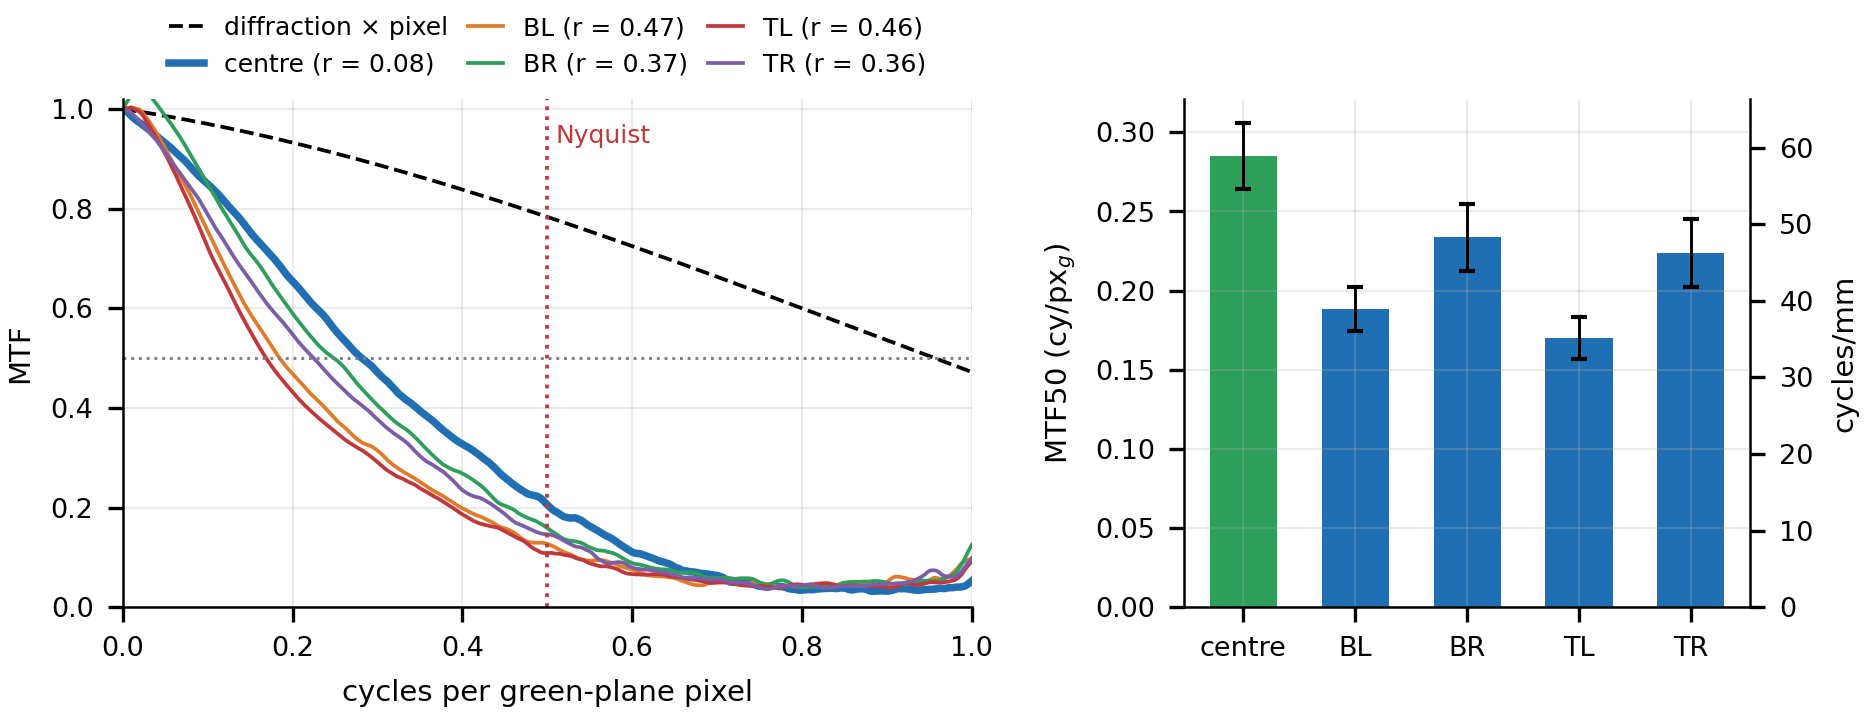
\includegraphics[width=0.92\linewidth]{figures/mtf_field.png}
\captionof{figure}{Left: mean MTF of each square and the diffraction $\times$ pixel prediction. Right: MTF50 per square reported as mean over captures.}
\end{center}

%======================================================================
\section{Noise: the Poisson--Gaussian Model}
\begin{textfig}[0.56]{noise_ptc.png}{Photon transfer curve,pairs and single frames.}
Ten pairs of flat fields at ISO 64 and 1/8s (above the 1/50 s flicker limit) were captured varying the light level of each pair. The two frames in each pair agreed within 0.09\,\% in their mean. To avoid lens shading, a 128x128 patch in the center of the green plane was analyzed. The signal mean was calculated as the average of the two frames minus the black level. Variance was calculated from the frame difference $\tfrac12\,\mathrm{Var}[A-A']$ to isolate temporal noise. Then, a weiighted linear fit of variance against mean was ran for the 8 pairs sitting below 70\,\% of full scale.

\textbf{Result.} $K$ = 0.273\,$\pm$\,0.014 DN/e$^-$, $\sigma_r$ = 6.7\,$\pm$\,0.6 e$^-$. The fit intercept, 3.32 DN$^2$, matches the variance measured directly in a 2 ms dark frame, providing an independent check of the read noise. The SNR follows the $\mu/\sqrt{\mu+\sigma_r^2}$ curve through both regimes, with the knee at 45 e$^-$.

\textbf{Why pairs.} A single frame keeps the fixed pattern (PRNU and shading gradients). Because fixed pattern variance scales as signal$^2$, fitting a single frame biases $K$ by 9.1\,\%. Subtracting the paired frames cancels this pattern out. 

\begin{warn}
\textbf{The model is not exact here.} The iPhone's raw pipeline isn't a perfect shot noise with read noise system. The apparent gain $(\mathrm{var}-c)/\mathrm{mean}$ drifts from 0.243 to 0.351 DN/e$^-$ as signal increases. In that case the uncertainty for $K$ was inflated ($\pm$5\,\%) to account for this curvature. Apple's own NoiseProfile $K$ = 0.316 aligns with this high signal end. Their stated intercept at 12.6 DN$^2$ is 3.8$\times$ higher than our measured dark variance, making thei read noise spec look conservative.
\end{warn}
\end{textfig}
\textbf{Dark current} Roughly 8.4\,$\pm$\,0.4 e$^-$/s based on frame mean dark signals at 2ms, 40ms, and 1s. Temperature wasn't tracked so this should be treated as an order of magnitude estimate.
\par\medskip\begin{center}
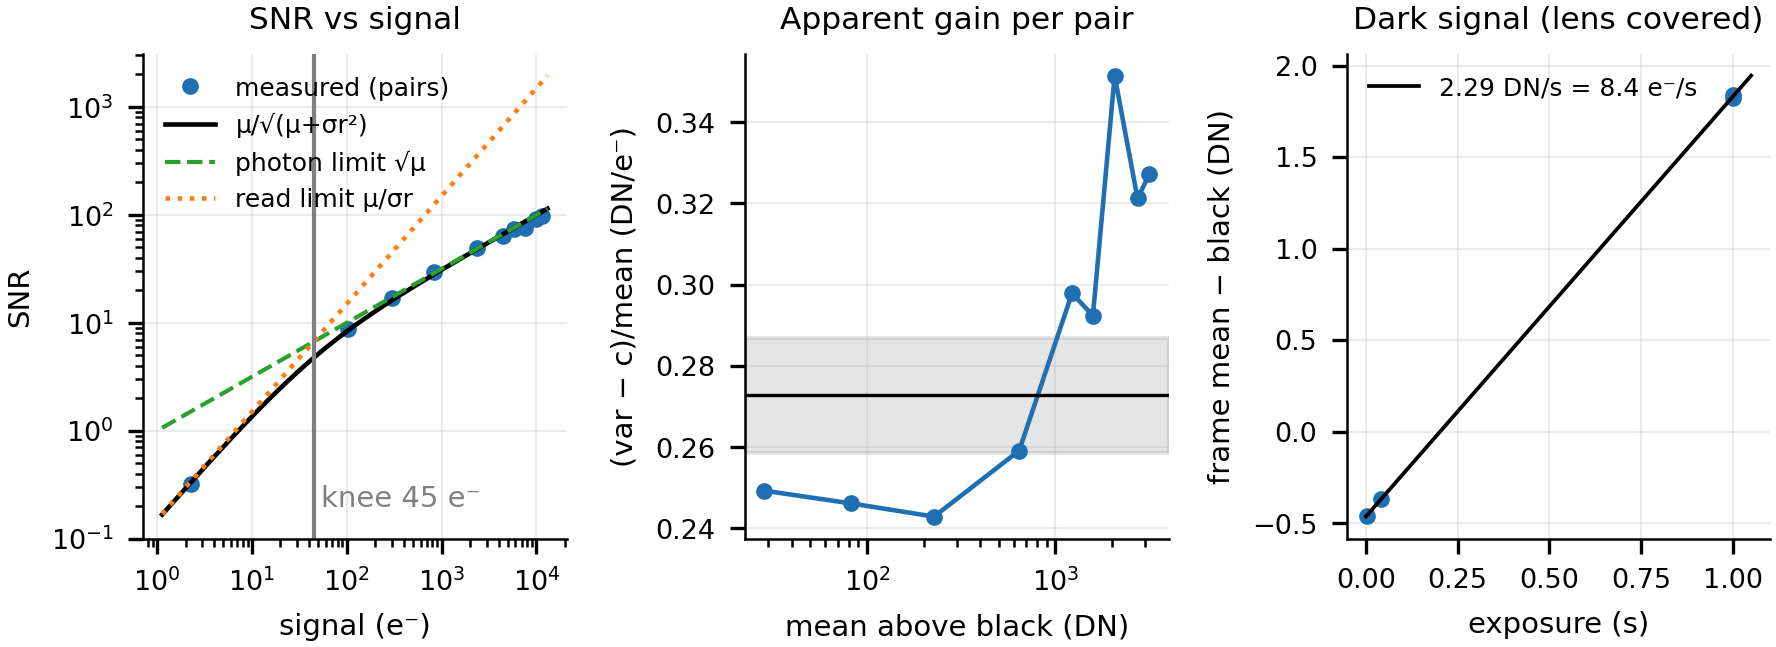
\includegraphics[width=0.88\linewidth]{figures/noise_snr_dark.png}
\captionof{figure}{SNR against the model; apparent gain per pair; dark signal against exposure.}
\end{center}

%======================================================================
\section{Dynamic Range}Setting the floor at the read noise DR = $(W-B)/\sqrt{c}$ = 10.93\,$\pm$\,0.09 stops (65.8\,$\pm$\,0.6 dB). Since the conversion gain $K$ cancels out in this ratio, that uncertainty depends purely on the intercept. If we define the floor strictly at SNR=1, the dynamic range drops slightly to 10.83 stops.

Note that the upper limit here is just where the 12-bit ADC clips, which isn't necessarily the physical full well capacity of the photodiode. Keep in mind therse figures are only valid for ISO 64; other test series were shot at ISO 100--400

%======================================================================
\section{Colour Accuracy}
\begin{textfig}[0.6]{color_sampling.png}{Chart 1 with the sampled region of each patch, numbered in reference order.}
During this test, three ColorChecker Classic Minis were sshot under identical room lighting at ISO 400 and 1/400 s, ensuring no pixels clipped (peak signal was 0.98 of full scale). After applying a shading correction using a white sheet from the same round, the 24 patches were automatically detected. We averaged the center of half of each patch directly from the quarter resolution raw data (one R, two G, one B per 2 $\times$ 2 tile) to avoid any interpolation artifacts. Chart orientation was determined by luminance rank and verified by making sure the neutral patches (19->24) correctly decreased in brightness.

For white balance, gains were calculated per channel using neural patch 5, resulting in gains of R 1.65 and B 3.30. Then, a Color Correction Matrix (CCM) was assembled using a 3 $\times$ 3 least squares fit from the balanced camera RGB to XYZ space.

\textbf{Reference.} Used colour-science values for the 2014 ColorChecker24 under a D50 illuminant, which matches charts and the published standard. CIEDE 2000 was established as the error metric with reference patch 19 serving as the Lab white point.
\end{textfig}
\textbf{Result.} The matrix drastically improved color accuracy, dropping the mean $\Delta E$ from 11.74,$\pm$,0.09 down to \textbf{2.45,$\pm$,0.11}. The worst individual patch improved from 19.5 (yellow-green) to 5.17,$\pm$,0.26 (purplish blue). After correction, the three worst patches fell in the saturated blue--cyan region: purplish blue (5.2), cyan (4.7), and blue (4.2). Because camera color filters don;t perfectly mimic human vision (no camera meets Luther condition), the error seen is inherent metamerism, not a bad mathematical fit. A matrix was trained on two charts and tested on the third to check for overfitting. The resulting error was 2.53,$\pm$,0.10, confirming good generalization. For comparison, applying Apple's built-in ForwardMatrix, interpolated to the 3169 K scene white per DNG specs, yielded a much higher error of 6.32,$\pm$,0.12. Apple's matrix handles neutrals excellently but struggles on saturated colors. This can explain why they choose to add LookTable profiles in their pipelines.

\par\medskip\begin{center}
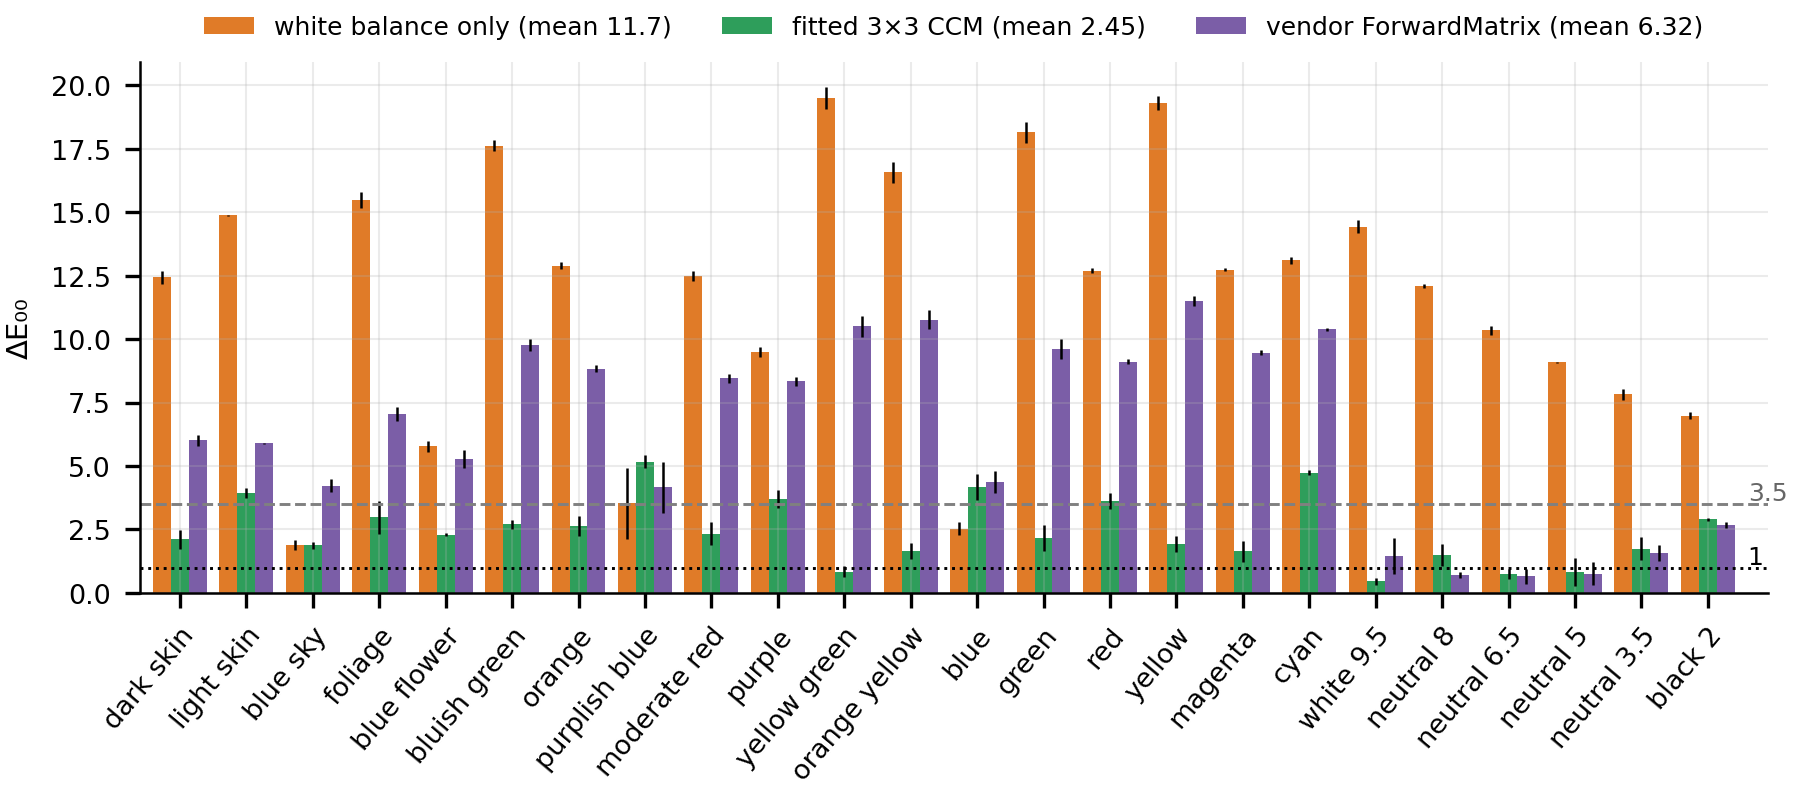
\includegraphics[width=0.8\linewidth]{figures/color_delta_e.png}
\captionof{figure}{CIEDE2000 in each patch. Dotted: 1 (just noticeable); dashed: 3.5 (visible at a glance).}
\end{center}
{\scriptsize\centering
\begin{minipage}[t]{0.49\linewidth}\centering
\begin{tabular}{@{}rlccc@{}}\toprule
\# & Patch & WB only & CCM & Apple FM \\ \midrule
1 & dark skin & 12.4\,$\pm$\,0.2 & 2.11\,$\pm$\,0.38 & 6.0\,$\pm$\,0.2 \\
2 & light skin & 14.9\,$\pm$\,0.0 & 3.94\,$\pm$\,0.20 & 5.9\,$\pm$\,0.0 \\
3 & blue sky & 1.9\,$\pm$\,0.2 & 1.88\,$\pm$\,0.14 & 4.2\,$\pm$\,0.2 \\
4 & foliage & 15.5\,$\pm$\,0.3 & 2.98\,$\pm$\,0.64 & 7.0\,$\pm$\,0.3 \\
5 & blue flower & 5.8\,$\pm$\,0.2 & 2.30\,$\pm$\,0.05 & 5.3\,$\pm$\,0.3 \\
6 & bluish green & 17.6\,$\pm$\,0.2 & 2.70\,$\pm$\,0.17 & 9.8\,$\pm$\,0.2 \\
7 & orange & 12.9\,$\pm$\,0.1 & 2.64\,$\pm$\,0.40 & 8.8\,$\pm$\,0.1 \\
8 & purplish blue & 3.5\,$\pm$\,1.4 & 5.17\,$\pm$\,0.26 & 4.2\,$\pm$\,1.0 \\
9 & moderate red & 12.5\,$\pm$\,0.2 & 2.34\,$\pm$\,0.47 & 8.4\,$\pm$\,0.2 \\
10 & purple & 9.5\,$\pm$\,0.2 & 3.70\,$\pm$\,0.37 & 8.3\,$\pm$\,0.2 \\
11 & yellow green & 19.5\,$\pm$\,0.4 & 0.83\,$\pm$\,0.22 & 10.5\,$\pm$\,0.4 \\
12 & orange yellow & 16.6\,$\pm$\,0.4 & 1.66\,$\pm$\,0.33 & 10.8\,$\pm$\,0.4 \\
\bottomrule\end{tabular}
\end{minipage}\hfill
\begin{minipage}[t]{0.49\linewidth}\centering
\begin{tabular}{@{}rlccc@{}}\toprule
\# & Patch & WB only & CCM & Apple FM \\ \midrule
13 & blue & 2.5\,$\pm$\,0.3 & 4.18\,$\pm$\,0.50 & 4.4\,$\pm$\,0.4 \\
14 & green & 18.1\,$\pm$\,0.4 & 2.16\,$\pm$\,0.53 & 9.6\,$\pm$\,0.4 \\
15 & red & 12.7\,$\pm$\,0.1 & 3.62\,$\pm$\,0.32 & 9.1\,$\pm$\,0.1 \\
16 & yellow & 19.3\,$\pm$\,0.3 & 1.93\,$\pm$\,0.31 & 11.5\,$\pm$\,0.2 \\
17 & magenta & 12.7\,$\pm$\,0.1 & 1.64\,$\pm$\,0.41 & 9.5\,$\pm$\,0.1 \\
18 & cyan & 13.1\,$\pm$\,0.1 & 4.74\,$\pm$\,0.11 & 10.4\,$\pm$\,0.1 \\
19 & white 9.5 & 14.4\,$\pm$\,0.3 & 0.45\,$\pm$\,0.14 & 1.5\,$\pm$\,0.7 \\
20 & neutral 8 & 12.1\,$\pm$\,0.1 & 1.49\,$\pm$\,0.43 & 0.7\,$\pm$\,0.1 \\
21 & neutral 6.5 & 10.3\,$\pm$\,0.2 & 0.75\,$\pm$\,0.20 & 0.7\,$\pm$\,0.3 \\
22 & neutral 5 & 9.1\,$\pm$\,0.0 & 0.84\,$\pm$\,0.55 & 0.8\,$\pm$\,0.4 \\
23 & neutral 3.5 & 7.8\,$\pm$\,0.2 & 1.75\,$\pm$\,0.45 & 1.6\,$\pm$\,0.3 \\
24 & black 2 & 7.0\,$\pm$\,0.1 & 2.90\,$\pm$\,0.06 & 2.7\,$\pm$\,0.1 \\
\bottomrule\end{tabular}
\end{minipage}\par}
{\footnotesize\centering Per-patch $\Delta E$, mean $\pm$ std over the three charts.\par}

%======================================================================

\clearpage
\section*{Decisions and Verification}
\subsection{Decided and rejected}
\begin{itemize}
\item \textbf{Measure straight from the raw green plane, not the demosaiced image.} DEmosaicing means you are measuring the interpolation algorithm instead of the actual sensor. A recognized trade-off is that MTF units end up as cycles per green plane pixel (Nyquist at 0.5), which is reported everywhere.

\item \textbf{Report the larger uncertainty (OpenCV's $\sigma$ vs jackknife $\sigma$) for all intrinsic parameters } The jacknife approach caught a significant variance in $f_x$ (14.1 vs 2.8 px) that was driven entirely by a single outlier view (\texttt{calib\_target016.dng}).


\item \textbf{Derive pixel pitch from the 35 mm equivalent focal length (2.420 $\mu$m), rather than calibration$f_\mathrm{mm}/f_\mathrm{px}$ (2.31 $\mu$m).} The calibration approach is skewed by focus breathing, since the lens to sensor distance increases by 1.9\,\% at a 0.36 m focus distance. Plus, since both calculations pull the focal length from the EXIF data anyway, the agreement wouldn't expose an error in the EXIF.

\item \textbf{Extract noise statistics from frame pair differences using a 128$^2$ center patch, keeping signals below 70\,\% of full scale.} Running the math on single frames artificially inflated $K$ by 9.1\,\%, and using the whole frame would have ruined the statistics by mixing in lens shading gradients.

\item \textbf{White balance on neutral patch 5, not the brightest white patch} The white patch from a few tests was carrying too much clipping risk. Three separate charts were shot to properly estimate uncertainty and validated the matrix with a test where we leave one chart out.
\end{itemize}

\subsection{Verification}
\begin{itemize}
\item \textbf{Unit tests against known ground truths} Verified synthetic Gaussian edges and ran a synthetic rotated square through the entire square finder pipeline. Additionally, a simulated sensor was built with shot noise, read noise, and PRNU. This hleped recover $K$ and prove the prediction that single frame $K$ estimates are biased high. Synthetic board calibrations were also tested and proving that $\sigma$,, rather than RMS correctly flags parallel views.

\item \textbf{Independent numbers that actually line up} The PTC intercept precisely matches the measured dark frame variance. The calculated principal point sits just (7.4, 6.6 px) away from Apple's official lens shading center and the three separate color charts agree within $\pm$0.11 $\Delta E$.

\end{itemize}

\subsection{Failures I found}
\begin{itemize}
\item The first automatic ROI on the bottom-right square returned NaN in 4 of 10 captures: the ROI reached the printed text beside the square and the LSF peak landed on the ROI border. I narrowed the ROI to 0.4 $\times$ the side and restricted the peak search to $\pm$8 px of the fitted edge; a test now covers the square pipeline.
\item In Exercise 2 a whole-row centroid returned MTF50 = 0.053 instead of 0.187 c/px on a synthetic edge, with no error raised; the windowed centroid fixed it, and the test keeps it fixed.
\item MTF scatter across captures is about 2$\times$ the photon-noise prediction, and the edge angle changed by 0.65$^\circ$: the ``repeat'' captures were not identical.
\item The PTC is curved (apparent gain 0.24 $\to$ 0.35); I inflated the gain uncertainty rather than quoting the 0.5\,\% a straight-line fit implies.
\end{itemize}

\subsection{AI tools}
Claude was used for the clarification of some concepts explored for this report. Moreover, the Latex organization was handled using AI for clear distribution of space and formatting. Table formatting was done using an AI tool and data comes directly from tests done in the jupyter notebooks of this repository. Plots and code is fully made by the author of the report and functions that were designed and verified using AI tools are described in each jupyter notebook. Grammar and paragraph eloquence were diagnosed by AI and suggestions were taken into consideration.

\subsection{What needs some further understanding}
\begin{itemize}
\item The MTF and distortion in the true frame corners.
\item Why the raw gain drifts with signal.
\item How to perform Dark current correct measurements.
\item How much of the Apple matrix's error the profile they add to the pipeline removes.
\end{itemize}

\section*{Resume Line}
Built an open source Python camera characterization toolkit (slanted-edge MTF, photon-transfer noise model, color correction, lens distortion), validated by tests against analytic ground truth, and published a measured datasheet with uncertainties for the iPhone 17 Pro Max main camera.

\end{document}
